\chapter{Machine Learning}
\label{chap:ml}

This section outlines the basic methodology followed in machine
learning research for Natural Language Processing. I will briefly
discuss machine learning from a general point of view and then present
supervised machine learning in more detail using linear regression as
example. I will then elaborate on the different kinds of classifiers
applied in NLP; both unstructured and structured.

\paragraph{Supervised and Unsupervised ML} There exists a broad
division of the field of machine learning into three sub-fields.
\begin{enumerate}
\item In {\it supervised} machine learning the aim is to learn a mapping
  from inputs $x$ (such as sentences) to outputs $y$ (such as
  morphological label sequences). To this aim, a supervised system
  uses training material consisting of input-output pairs $(x,y)$ and
  a model which can represent the mapping $x \mapsto y$. Training of
  the model consists of tuning its parameters in such a way that the
  model accurately describes mapping between the inputs and outputs in
  the training data. Typically, supervised machine learning is
  employed for tasks such as classification and regression. Examples
  in the field of natural language processing include POS tagging and
  other tasks that can be framed as labeling (for example named entity
  recognition), speech recognition and machine translation.
\item In contrast to supervised machine translation, {\it unsupervised}
  approaches exclusively utilize unannotated data, that is the
  training data consists solely of inputs $x$. Unsupervised machine
  learning is most often used for various kinds of clustering tasks
  where inputs are grouped into sets of similar examples. Therefore,
  it has applications for example in exploratory data analysis.
\item Finally, {\it semi-supervised}
  systems use an annotated training set in combination with a,
  typically, very large unannotated training set to improve the
  results beyond the maximum achievable by either approach in
  isolation.
\end{enumerate}

Unsupervised and Semi-supervised techniques have many applications in
the field of tagging. For example, distributional similarity can be
used to improve tagging accuracy for OOV words
\citep{Huang2009a,Ostling2013} and self-training can improve the
accuracy of a tagging system \citep{Spoustova2009,Sogaard2011}.  This
thesis, however, focuses exclusively on supervised learning.

\section{Supervised Learning}
%\begin{itemize}
%\item Example: linear regression.
%\item Estimation from a sample.
%\item Convexity, smoothness.
%\item Regularization.
%\item Methodology: Training, development and test sets. 
%\item Significance testing.
%\end{itemize}

In this section, I will illustrate the key concepts and techniques in
supervised machine learning using the very simple example of {\it
  linear regression}. I will explain the plain linear regression model
and show how it can be fitted using training data. I will then briefly
present {\it ridge regression} which is a {\it regularized} version of
linear regression.

I choose linear regression as example because it is a simple model yet
can be used to illustrate many important concepts in machine
learning. Moreover, the model has several tractable properties such as
smoothness and convexity. Additionally, it can be seen as the simplest
example of a linear classifier which is a category of models
encompassing conditional random fields, the hidden Markov model and
average perceptron classifier presented in later chapters.

\paragraph{Linear Regression} As a simple example, imagine a person
called Jill who is a real estate agent.\footnote{This example is
  inspired by the Machine learning course provided by Coursera and at
  the time taught by Andrew Ng.} She is interested in constructing an
application, for use by prospective clients, which would give rough
estimates for the selling price of a property. Jill knows that a large
number of factors affect housing prices. Still, there are a few very
robust predictors of price that are easy to measure.
She decides to base the model on the following predictors:
\begin{enumerate}
\item The living area.
\item The number of rooms.
\item The number of bathrooms.
\item Size of the yard.
\item Distance of the house from the city center.
\item Age of the house.
\item Amount of time since the last major renovation.
\end{enumerate}

Jill decides to use the simplest model which seems reasonable. This
model is linear regression which models the dependent
  variable, the house price, as a linear combination of the independent
variables listed above and parameter values in $\R$. The linear
regression model is probably not accurate. It fails in several
regards. For example, increasing age of the house probably reduces the
price up to a point but very old houses can in fact be more expensive
then newly built houses especially if they have been renovated lately.
Although, the linear model is unlikely to be entirely accurate, Jill is
happy with it because the intention is just to give a ball park
estimate of the price for the prospective client.

To formalize the linear regression model, let us call the dependent
variable price $y$ and each of the independent variables living area,
number of rooms and so on $x_i$. Given a vector $x = (x_1, ...,
x_n, 1)^\top \in \R^n$, which combines the independent
variables $x_i$, a bias term $1$, and a parameter vector $\theta \in
\R^{n+1}$ the linear regression model is given by Equation
\ref{eq:linreg}.\footnote{In reality, each of the predictors would probably
  be transformed to give all of them the same average and
  variance. Although this ii not required in theory, it tends to give
  a better model.}

\begin{equation}
y(x\parcond \theta) = x^\top\theta\label{eq:linreg}
\end{equation}

Two questions immediately arise: How to compute the price given
parameters and predictors and how to compute the parameter vector
$\theta$. These questions are common for all supervised learning
problems also when using other models than the linear regression
model.

\paragraph{Inference} The first question concerns {\it inference},
that is finding finding the values of the dependent variable given
values for the independent variables. In the case of linear
regression, the answer to this question is straightforward. To compute
the price, simply perform the inner product in Equation
\ref{eq:linreg}. The question is, however, not entirely settled
because one might also ask for example how close to the actual price
the estimate $y$ is likely to be. A related question would be to
provide an upper and lower bound for the price so that the actual
price is very likely to be inside the provided bounds. To answer these
questions, one would have to model the expected error.

Inference is very easy and also efficient in the case of linear
regression. With more complex models such as structured graphical
models which are investigated in Chapters \ref{chapter:hmm} and
\ref{chapter:crf}, it can however be an algorithmically and
computationally challenging problem. The task is still the
same: Find the $y$ which is most likely given the input.

\paragraph{Training Data} The second question concerns {\it estimation
  of model parameters} and it is more complex than the question of
inference. First of all, Jill needs training data.  In the case of
house price prediction, Jill can simply use data about houses she has
brokered in the past. She decides to use a training data set
$\mathcal{D} = \{(x^1, y^1), ..., (x^T, y^T)\}$, where each $x^t =
(x^t_1\ ...\ x^t_n\ 1)$ is a vector of independent variable values
(living area, age of the house and so on) and $y^t$ is the dependent
variable value, that is the final selling price of the house. The last
element $1$ in $x^t$ is the bias which is constant. Now Jill needs to
make a choice. How many training examples $(x^t, y^t)$ does she need?
The common wisdom is that more data is always better. In practice, it
is a good idea to start with a small training data and increase the
number of training examples until the performance of the system
plateaus.

\paragraph{Data Sparsity} Whereas it is fairly easy to get a
sufficient amount of training data for our example which only has a
few parameters, it is vastly more difficult to accomplish with more
complicated models in natural language processing. When there is
insufficient data to estimate model parameters accurately, the data is
called sparse. One central question in this thesis is how to
counteract {\it data sparsity} in morphological tagging.

\paragraph{Loss Functions} The objective in estimation is to find a
parameter vector $\theta$ which in some sense minimizes the error of
the house price predictions $y(x^t\parcond \theta)$ when compared to
the actual realized house prices $y^t$ in the training data. The usual
minimization criterion used with linear regression is the least square
sum criterion given in Equation \ref{eq:lss}. It is minimized by a
parameter vector $\theta$ which gives as small square errors $|y^t -
y(x^t \parcond \theta)|^2$ as possible.

\begin{equation}
\theta = \argmin_{\theta' \in \R^n} \sum_{x^t \in \mathcal{D}} | y^t - y(x^t\parcond \theta')|^2\label{eq:lss}
\end{equation}

The square sum is an example of a {\it loss function} (also called the
objective function). A loss function assigns a non-negative real loss
for each parameter vector. Using the concept of loss function, the
objective of estimation can be reformulated: Find the parameter vector
$\theta$ that minimizes the average loss over the training data.

%\paragraph{The Exact Solution} In the case of linear regression, there
%is a well known exact solution for $\theta$ which utilizes linear
%algebra. The solution is given in Equation \ref{eq:lss-exact}. The
%matrix $X \in \R^T_n$ is defined by $X_{t,i} = x_t[i]$ and its
%More-Pennrose pseudoinverse $X^+ \in \R^n_T$ is defined as $X^+ =
%(X^\top X)^{-1}X^\top$. The vector $Y \in R^T$ is simply the vector of
%realized house prices $y_t$. The solution $\theta$ exists only when
%none of the independent variables are linear combinations of each
%other in the training data.

%\begin{equation}
%\theta = X^+ Y \label{eq:lss-exact}
%\end{equation}

\paragraph{Iterative Estimation} In the case of linear regression
model, there is an exact solution for the optimization of parameter
vector $\theta$.\footnote{The solution is given by $\theta = X^+Y$
  where $X^+ = (X^\top X)^{-1}X^\top$ is the More-Pennrose
  pseudo-inverse of $X$.} This does not hold for more complex
models. Moreover, the exact solution might often not be the one that
is desired because it does not necessarily generalize well to unseen
examples. This is called {\it over-fitting}. Fortunately, the loss
function can be modified to counteract over-fitting. After the
modification, the parameter optimization problem might, however, no
longer have a closed form solution.

Because the loss of the training data is a function of the model
parameters, one can apply analytical methods to try to find optimal
parameter values. These methods include for example Newton's method
which is an iterative procedure that can be used to find the zeros of
a differentiable function or local extrema of a twice differentiable
function. Approximations of Newton's method, so called Quasi-Newton
methods \citep{Liu1989}, have also been developed because Newton's
method requires evaluation and inversion of the Hessian matrix of a
function. This is a very costly operation for functions where the
domain has high dimension. Quasi-Newton methods use approximations of
the inverse Hessian.

A simpler method called gradient descent can be applied to functions
that are once differentiable. In
general, gradient descent converges toward the optimum more slowly
than Newton's method, however, the computation of one step of the
iterative process is much faster when using gradient
descent. Therefore, it may be faster in practice.

All gradient based methods rely on differentiability of the loss
function.\footnote{At least, differentiability almost everywhere.} For
the models used in this thesis, differentiability holds. Gradient
based methods work in the following general manner. Let
$\mathcal{L}_{\mathcal{D}}:\R^n \rightarrow \R$ be the loss of the training data
$\mathcal{D}$.

\begin{enumerate}
\item Start at a random point $\theta_0$ in the parameter space.
\item Determine the direction of steepest descent of the loss
function. This is the negative gradient $-\nabla
\mathcal{L}_{\mathcal{D}}(\theta_t)$ at point $\theta_t$.\label{alg:dir}
\item Determine a suitable step size $\alpha_t \in \R_+$.
\item Take a step of length $\alpha_t$ in direction $v_t$ to get to
the next point in the parameter space $\theta_{t+1}$, that is
$\theta_{t+1} = \theta_t - \alpha_t \nabla \mathcal{L}_{\mathcal{D}}(\theta_t)$.
\item If the difference in loss $|\mathcal{L}_{\mathcal{D}}(\theta_{t+1}) -
\mathcal{L}_{\mathcal{D}}(\theta_t)|$ is smaller than a threshold $\rho$, set
$\theta = \theta_{t+1}$. Otherwise, set $\theta_t = \theta_{t+1}$ and
return to line \ref{alg:dir}.
\end{enumerate}

The main difference between first and second order methods is the
computation of the step size $\alpha_t$. Second order methods can take
longer steps when the loss is plateauing. Thus they typically take
fewer steps in total. In first order methods such as gradient descent,
$\alpha_t$ can be constant, a decreasing function of $t$ or can also
be determined by a line search in the direction of $-\nabla
\mathcal{L}_{\mathcal{D}}(\theta_t)$. For example $\alpha_t =
t^{-1}$ may work.\footnote{In general, stepsize $(\alpha_t)_{t \in
\N}$ that resemble the harmonic sequence, that is $\sum \alpha_t^2 <
\infty$ and $\sum \alpha_t = \infty$, guarantee convergence of
gradient descent to an minimum of the loss function (if it exists) for
a wide variety of functions \cite{someone}}


As the meta-algorithm above suggests, gradient based optimization
algorithms are local in the sense that they always move in the
direction of steepest descent of the loss function, that is toward a
local optimum. Therefore, they will in general not find the global
optimum of the loss function. By choosing a {\it convex} loss
function, which has maximally one local, and thus also, global optimum it
is possible to avoid getting stuck at local optima.

Convexity is, however, not enough to guarantee convergence to a global
optimum. First of all, a global optimum might not exist.\footnote{This
can happen if the domain of the loss function is not
compact. Unfortunately, it usually is not.} Moreover, convergence may be
too slow. This can leads to premature termination of the training
procedure. This is specifically a problem for first order methods.

\paragraph{Online Estimation} The optimization methods
discussed up to this point have been so called {\it batch
  methods}. The derivatives of the loss function is computed over the
entire training data and parameters are updated accordingly. Batch
methods can be slow and subsequent training when new training examples
become available is computationally intensive. {\it Online algorithms}
are an alternative to batch methods, where the loss is instead
computed for a randomly chosen training example and the parameters are
the updated accordingly. In practice, online methods
can give fast convergence. Moreover, re-training is relatively
efficient when new training examples become available.

{\it Stochastic gradient descent} is a well known online estimation
algorithm. In practice, it converges faster than regular gradient
descent \cite{someone} but is identical in all other respects except
that it is an online estimation algorithm instead of a batch
algorithm. The algorithm processes one random training example at a
time. It uses the gradient $\nabla L_{\mathcal{D}[i]}(\theta)$ of the
loss over the single training example $\mathcal{D}[i]$ to approximate
the gradient $\nabla L_{\mathcal{D}}(\theta)$ for the entire training
data $\mathcal{D}$. 

%She also needs to
%decide upon an {\it estimator}, that is, a method for setting the
%parameters $\theta$.

\paragraph{Regularization} Due to the problem of over-fitting, a
family of heuristic techniques called {\it regularization} is often
employed. They aim to transform the original problem in a way which
will penalize both deviance from the gold standard and ``complexity''
of the solution $\theta$. Regularization can be seen to convey the
same idea as Occam's Maxim which states that a simpler explanation for
a phenomenon should be preferred when compared to a more complex
explanation yielding equivalent results. Of course, this does not
explain what is meant by a ``complex'' parameter vector
$\theta$.

To illustrate simple and complex parameter vectors, examine a case of
linear regression where the dependent variable $y$ and the predictors
$x_i$ have mean $0$ and variance $1$ in the training data. This may
seem restrictive but in fact any linear regression problem can easily
be transformed into this form by applying an affine transformation $z
\mapsto az - b$. When doing inference, this affine transformation can
simply be reversed by applying $z \mapsto a^{-1} (z + b)$. The
simplest parameter vector $\theta$ is clearly the zero vector $\theta
= (0 ... 0)^\top$. It corresponds to the hypothesis that the
predictors $x_i$ have no effect on the dependent variable
$y$. According to this hypothesis, the prediction for the house price
is identically zero.

The zero solution to a linear regression problem is simple but also
completely biased. Because we are assuming that the independent
variables $x_i$ explain the dependent variable $y$, a model that
completely disregards them is unlikely to give a good fit to the
training data. By introducing a regularization term into the loss
function, we can however encourage simple solutions while at the same
time also preferring solutions that give a good fit. There are several
ways to accomplish this but the most commonly used are so called $L_1$
and $L_2$ regularization.\footnote{Another approach to counteracting
  over-fitting is provided by Bayesian statistics where the parameter
  vector $\theta$ is drawn from a prior distribution. In practice,
  Bayesian methods and regularization are often equivalent.} These are
general regularization methods that are employed in many models in
machine learning.

The $L_1$ regularized loss function for linear regression is given in
Equation \ref{eq:lss-l1}. $L_1$ regularization, also called LASSO
regularization \cite{Tibshirani1996}, enforces solutions where many of
the parameter values are $0$ (such parameter vectors are called
sparse). It is suitable in the situation where the model is over
specified, that is, many of the predictors might not be necessary for
good prediction. The $L_1$ regularized linear regression loss is given
by Equation \ref{eq:lss-l1}.

\begin{equation}
\theta = \argmin_{\theta' \in \R^n} \sum_{x_t \in \mathcal{D}} | y^t - y(x^t\parcond \theta')|^2 + \lambda \sum_i |\theta_i|\label{eq:lss-l1}
\end{equation}

The $L_2$ regularized loss function is given in \ref{eq:lss-l2}. $L_2$
regularization is also called Tikhonov regularization. In contrast to
$L_1$ regularization, it directly prefers solutions with small norm. A
linear regression model with Tikhonov regularization is called a ridge
regression model.

\begin{equation}
\theta = \argmin_{\theta' \in \R^n} \sum_{x_t \in \mathcal{D}} | y_t - y(x_t\parcond \theta')|^2 + \lambda \|\theta\|^2 = \argmin_{\theta' \in \R^n} \sum_{x_t \in \mathcal{D}} | y_t - y(x_t\parcond \theta')|^2 + \lambda \sum_i |\theta[i]|^2\label{eq:lss-l2}
\end{equation}

The coefficient $\lambda \in \R^+$ is called the {\it
  regularizer}. The regularizer determines the degree to which model
fit and simplicity affect the loss. A higher $\lambda$ will increase
the loss for complex models more than a lower one. When $\lambda$
increases, the optimal parameter vector $\theta$ approaches the zero
vector and when it decreases $\theta$ approaches the parameters that
fit the training data as closely as possible. This is called
under-fitting.

\paragraph{Hyper-parameters} The regularizer is a so called {\it hyper-parameter} of the
regularized liner regression model. It is easy to see that increasing
$\lambda$ will automatically increase the loss. Therefore, there is no
direct way to estimate its correct magnitude simply using the training
data. Instead {\it held-out data} can be used. Held-out data is
labeled data that is not used directly for estimating model
parameters. If the model over-fits the training data, that is
generalizes poorly to unseen examples, the held-out data will have a
high loss. However, it will also have a high loss if the model
under-fits, that is, performs poorly on all data. Held-out data can
therefore be used to find an optimal values for the regularizer
$\lambda$. Often one tries several potential values and chooses the
one that minimizes the loss of the held-out data. Usually, one uses
the unregularized loss function for the held-out data.

\section{Machine Learning Experiments}

In this thesis and in the associated articles, I present several
experiments in morphological tagging. The experiments are conduct on
labeled data and follow a set pattern.

\begin{enumerate}
\item {\bf Data Splits} The labeled data set is divided into
  three non-overlapping parts: (1) a training set used for estimating
  model parameters (2) a development set used for setting hyper
  parameters and performing preliminary experiments during development
  and (3) a test sets which is used to perform the final evaluation of
  the model.
\item {\bf Feature Engineering} Using the training set and development
  set, a number of features are tested and depending on tagging errors
  in the development data, new features may be added.
\item {\bf Tuning} The model hyper-parameters are set using
  development data.
\item {\bf Training} When model parameters and hyper-parameters are
  set, the model is trained. Training time is measured at this point.
\item {\bf Evaluation} The performance of the model is measured on the
  test data in order to derive an estimate of tagging accuracy and
  tagging speed.
\end{enumerate}

A crucial component of machine learning experiment is the
baseline. For example, when investigating the impact of a set of
features on tagging accuracy, the baseline will be the model which
does not include those features. When investigating the tagging
accuracy, tagging speed or training speed of the FinnPos toolkit, the
baseline will be another established tagger toolkit.

When comparing tagging accuracy of two taggers, we compare their
accuracies on the test set. However, this is only an estimate of the
true tagging accuracies of the systems. When the difference in
performance between the systems is small, it is therefore not possible
to say with great certainty which system will perform better on new
data. In this situation, it is helpful to know about the variance of
the accuracy. 

The variance is a measure of the stability of the difference in
accuracies between tagging systems. It can be estimated using random
samples of the test data. If one system consistently performs better
than the other one on random samples of the test data, it is more
likely to performs better on some unseen sample. In contrast, when the
performance of one system is better on some samples and worse on
others, it is less certain that it would perform better on unseen data
even though it performs better on average in the entire test set.

Using statistical significance testing, the above comparison can be
formalized. In the papers included in this thesis, the 2-sided
Wilcoxon signed-rank test \citep{Wilcoxon45}. In contrast to the often
used t-test, the Wilcoxon test does not assume that the measurements
are drawn from a Gaussian distribution. A 2-sided test (instead of a
1-sided test) is used because it cannot be known which of the systems
actually has the higher accuracy although we know that one of the
systems performs better on the test set.\footnote{This was suggested
  by one of the reviewers of Publication \ref{pub:6}.}

%\begin{itemize}
%\item Evaluation metric.
%\item Training set, development set, test set.
%\item Significance of results.
%\item Estimating variance.
%\item Statistical significance testing.
%\end{itemize}

%\section{Classification}
%\begin{itemize}
%\item Naïve Bayes' classifier.
%\item Generative and Discriminative Classifiers.
%\item Linear classifiers: logistic classifier, perceptron classifier \citep{Freund1999},
%  SVM \citep{Cortes1995}.
%\end{itemize}

%The main topic of this thesis is morphological tagging. It can be seen
%as a structured {\it classification task} where each word in a
%sentence is assigned one morphological label.\footnote{which may have
%  internal structure as is seen in Section
%  \ref{sec:sub-labels}.} Classification is a fundamental supervised
%machine learning task where the objective is to learn a mapping from
%objects like words, sentences, documents or images onto discrete
%classes such as morphological labels (Noun+Sg+Nom) or sentiments
%(Positive sentiment versus Negative Sentiment).

%Classification resembles regression. The output of a classifier is, however, not
%a single real value $y$ but a distribution over the set of nominal
%classes.

%Probabilistic classifiers can broadly be divided into two groups,
%namely generative and discriminative. Generative classifiers learn a
%joint distribution $p(x,y)$ over labels $y$ and input examples
%$x$. Given an example $x$, a distribution over classes $y$ can be
%computed using the marginal probability of example $x$, which is $p(x)
%= \sum_{y' \in Y} p(y',x)$. The probability distribution over classes
%is defined by $p(y|x) = p(y,x) / p(x)$.

%\section{Structured Classifiers}
%\begin{itemize}
%\item The idea of chained stochastic processes.
%\item Markov chain.
%\item HMM
%\item MEMM
%\item CRF
%\end{itemize}

%There are tasks in natural language processing that cannot be
%adequately formulated as supervised classification tasks in the simple
%way that has been discussed earlier. Examples of tasks that require
%more sophisticated methods are syntactic parsing and translation
%between languages. One could think of parsing as a labeling task where
%the objective is to label a sentence with the appropriate syntactic
%tree. Likewise, the translation of a sentence could be seen as its
%label. 

%It is, however, easy to see that these approaches are deeply
%flawed. Firstly, there is an infinite number of syntactic trees and
%indeed an infinite number of sentences of finite length. Therefore,
%the label set would have to be infinite as well. Secondly, the data
%sparsity problem would be unmanageable. Just in order to see most
%relatively frequent syntax trees for moderately long English
%sentences, say twenty words long, we would need an unfathomable amount
%of training data.

%Instead of a simplistic classification approach, {\it structured}
%classifiers can be employed. Structured classifiers relate parts of
%the complex label such as a translation, syntax tree or sequential
%labeling with the input. They also learn how to piece together complex
%labels from simple constituents. A very simple (and probably very bad)
%translation software could learn how to translate isolated English
%words into French words and then learn how to combine French words
%into sentence as shown in Figure \ref{fr-tr}. Note that although both
%``Le'' and ``La'' are perfectly good translations for ``The'', only
%``Le'' is usually possible before ``chien'', which is a masculine
%French word.

%In general, structured classifiers rely on two models, the
%unstructured and structured model. The unstructured model learns to
%relate simple labels such as words in a translation or nodes in a
%syntax tree with the input. In contrast, the structured model learns
%how to combine simple labels into complex labels such as entire
%translations or syntax trees. In practice, some models make a stricter
%division then other models.

%Structured models are the main subject matter of this thesis and I
%will present two structured models, the Hidden Markov model and the
%Conditional random field in detail in Chapters \ref{hmm} and
%\ref{crf}.
 
%\begin{figure}
%\caption{A translation from English to French}\label{fr-tr}
%\begin{center}
%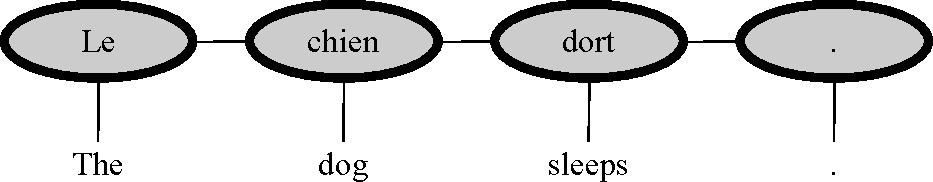
\includegraphics[scale=0.75]{chien}
%\end{center}
%\end{figure}

%\section{The Aim of Research -- Improving the State of the Art}
%
%Like most language technological research, the work documented in this
%thesis aims at improving existing solutions for language
%processing. Specifically, my work is targeted at improving
%morphological taggers for morphologically rich languages. It is not
%entirely easy to define what constitutes an improvement to the field
%of morphological tagging or indeed any sub-field of language
%technology. Nevertheless, most researchers would probably agree that
%the following kinds of changes are improvements compared to existing
%approaches:
%
%\begin{enumerate}
%\item Improving labeling accuracy.
%\item Speeding up estimation.
%\item Speeding up tagging.
%\item Reducing model size. \label{quant}
%\item Clarifying the underlying theoretical foundations.
%\item Simplifying implementation of taggers.
%\item Uncovering best practices for building taggers.
%\end{enumerate}
%
%Items 1 though \ref{quant} in the list above are {\it quantifiable}
%improvements. It is possible to perform experiments to measure the
%labeling accuracy, tagging speed, estimation speed and model size
%given by different morphological taggers and derive conclusions about
%the respective merits of the taggers. In contrast, the rest of the
%items in the list cannot be measured as easily. 
%
%Although, most probably would agree that clarifying theoretical
%foundations of a field is a substantial contribution, it may not be as
%easy to agree upon what constitutes a clarification. This could for
%example be dependent on the background of individual
%researchers. Similarly, one model might be more straight-forward to
%implement than another model using some programming language, however,
%this can very well depend on the specific programming language and
%available libraries to some degree.
%
%Because quantifiable improvements are easier to ascertain, this thesis
%focuses on demonstrating such improvements compared to other state of
%the art approaches. Nevertheless, I will also aim to show that the
%model demonstrated in the thesis is conceptually simpler than other
%state of the art approaches.
%
%Although quantifiable improvements are easier to demonstrate than
%other improvements, there are still caveats. First of all, it is
%impossible to compare machine learning models directly. One can only
%compare implementations of the models. Because of differences between
%platforms even different implementations of the exact same model can
%have radically different run time on the same data. Moreover, bugs in
%the implementation of different models can reduce the accuracy or have
%sporadic effects on run time.
%
%Besides practical concerns like dependence on implementation, there
%are also theoretical issues that interfere with measuring performance
%of different models. It is easy to say that the accuracy of one system
%is better than another system on {\it a specific data set}. This does,
%however, not imply that the accuracy is better on {\it all data
%  sets}. In formal terms, we can only conduct experiments on samples
%of the distribution of all texts in a given language. Therefore, our
%experiments will yield results only in a probabilistic sense: it is
%likely that the labeling accuracy of one system is better than the
%accuracy of another, if the accuracy was better on the sample used for
%testing.
% 
%Using large test sets and test sets compared from a variety of
%different genres will probably give more reliable results. This is,
%however, also to some extent a debatable matter. Some methods are very
%accurate on the same genre that they were trained on but perform worse
%on other genres. Other methods instead perform well on average but, as
%a trade-off, cannot reach as high accuracy on a specific text
%domain. It is not easy to say which kind of system is preferable. This
%trade-off is called the bias variance trade-off \cite{?} and it has
%bearing on measuring the performance difference of systems. 
%
%When using a high variance system, accuracy on different texts varies
%a lot. When instead using a system with high bias, the accuracy tends
%to vary much less.
%
%When comparing two systems, it is not sufficient to simply look at the
%performance of the systems on a test set. If we measure the
%performance of the systems on a particular test, one of them will
%almost certainly perform better than the other regardless of whether
%there is an actual difference in the performances of the systems. The
%probability of exactly equal performance is simply very small. 
%
%The larger the test sets are, the more accurately the results of
%experiments will on average reflect the true performance of the
%systems. This is easy to see, because ultimately the test set will represent the entire domain. Unfortunately, the amount of test material is usually
%restricted and producing more test data might not be
%feasible.\footnote{Especially when using standard data sets, one is
%  restricted to the given amount of test data}
%
%An approach that is often used is splitting the test data into
%segments and performing several experiments -- one for each
%segment. If one system outperforms the other system on most segments
%with a large margin, then we are more confident in saying that there
%is in fact a difference in the performance of the systems. If on the
%hand each system outperforms the other on roughly half of the
%segments, we might be inclined to doubt whether there is any real
%difference in performance between the systems. The higher the variance
%between the results, the larger the margins between the systems need
%to be in order for us to be able to conclude that there is a
%difference in performance. This argument can be made rigorous using
%statistical tests which measure the significance of the difference in
%performance of two systems.
%
%The usual set up of statistical significance testing is to make a null
%hypothesis $H_0$ that the average performance of two systems is the
%same. After this a test statistic is computed. The test statistic is
%simply a real number whose value indicates the significance of the
%difference in performances between the systems. If the statistic is
%high enough, the null hypothesis can be discarded in favor of the
%alternative hypothesis that there is a genuine difference in
%performance between the systems. The test statistic incorporates
%information about the difference in performance of the systems on test
%data all segments as well as the variance of the performances.
%
%In the work conducted presented in this thesis, I have used the
%Wilcoxon signed-rank test \cite{?} to ascertain the significance of
%results. I use it instead of the T-test because it is not dependent on
%the fact that the distribution of differences in performance are
%normally distributed.\footnote{In practice it might be a fairly
%  accurate assumption that the differences are normally
%  distributed. This often holds for measurements \cite{?}.} In
%practice it is less sensitive than the T-test.
%
